\documentclass[12pt]{article}
\usepackage{graphicx}
\usepackage{booktabs}
\usepackage[font=footnotesize,skip=5pt]{caption}
\usepackage[font=scriptsize,skip=0pt]{subcaption}
\usepackage{amsmath}
\usepackage{amsfonts}
\usepackage{amssymb}
\usepackage{lscape}
\usepackage{psfrag}
\usepackage[usenames]{color}
\usepackage{bbm}
\usepackage[update]{epstopdf}
\usepackage[bookmarks,pdfstartview=FitH,a4paper,pdfborder={0 0 0}]{hyperref}
\usepackage{verbatim}
\usepackage{listings}
\usepackage{textcomp}
\usepackage{course}
\usepackage{fancyhdr}
\usepackage{multirow}
\pagestyle{fancy}
\usepackage{tikz}
\usepackage{bm}
\usepackage{float}
%\usepackage{subfig}

\renewcommand{\sectionmark}[1]{\markboth{#1}{#1}}
\renewcommand{\subsectionmark}[1]{\markright{#1}}

\newtheorem{theorem}{Theorem}
\DeclareMathOperator{\Var}{Var}
\DeclareMathOperator{\Bias}{Bias}

\graphicspath{ {../../Images/} }
\usepackage[backend=biber, style=bwl-FU, sorting=nyt]{biblatex}
\addbibresource{bib.bib}

\fancyhf{}
\fancyhead[RO]{\nouppercase{\footnotesize\sc\leftmark\ \hrulefill\ \thepage}}
%\fancyhead[RE]{\nouppercase{\footnotesize\sc\thepage\ \hrulefill\ }}
\renewcommand{\headrulewidth}{0pt}

\makeatletter
\def\cleardoublepage{\clearpage\if@twoside \ifodd\c@page\else%
\hbox{}%
\thispagestyle{empty}%
\clearpage%
\if@twocolumn\hbox{}\clearpage\fi\fi\fi}
\makeatother


\renewcommand{\topfraction}{0.9}  % max fraction of floats at top
\renewcommand{\bottomfraction}{0.8} % max fraction of floats at bottom
% Parameters for TEXT pages (not float pages):
\setcounter{topnumber}{2}
\setcounter{bottomnumber}{2}
\setcounter{totalnumber}{4}            % 2 may work better
\setcounter{dbltopnumber}{2}           % for 2-column pages
\renewcommand{\dbltopfraction}{0.9}    % fit big float above 2-col. text
\renewcommand{\textfraction}{0.07}     % allow minimal text w. figs
% Parameters for FLOAT pages (not text pages):
\renewcommand{\floatpagefraction}{0.7}  % require fuller float pages
% N.B.: floatpagefraction MUST be less than topfraction !!
\renewcommand{\dblfloatpagefraction}{0.7} % require fuller float pages

\sloppy

\widowpenalty=10000
\clubpenalty=10000

\edef\today{%\number\day\
\ifcase\month\or
January\or February\or March\or April\or May\or June\or July\or
August\or September\or October\or November\or December\fi\ \number\year}
\title{\vspace*{40.0mm}
  \bf Report on project about clustering
         \vspace*{20.0mm} \\
  %\vspace{-20mm}\framebox{DRAFT VERSION}\vspace{20mm} \\
  \Large\bf Statistical Data Analysis 
  
 
  
  Project 2 \vspace*{20.0mm}
  \vspace*{40.0mm}}
\author{Mitja Mandić}
\date{ May 2022}

\begin{document}

\begin{figure}
  \parbox[t]{125mm}{
    \vspace*{6mm}
    \scriptsize\sf           DEPARTMENT OF MATHEMATICS \\
    \scriptsize\sf           FACULTY OF SCIENCE\\
    \scriptsize\sf           KU LEUVEN}
  \parbox[t]{40mm}{
    \begin{flushright}
      
\includegraphics[height=15mm]{../images/logo.eps.pdf}
    \end{flushright}}
\end{figure}

\maketitle
\thispagestyle{empty}
\raggedbottom

\cleardoublepage
\pagenumbering{roman}
\setcounter{tocdepth}{2}
%\tableofcontents
\pagenumbering{arabic}

\section{Introduction}
For the second project for the course Statistical Data Analysis we are once again worikng with the
dataset of spectral data of four cultivars of canteloupe melons. 

Groups we work in this report with were also again chosen randomly, with 50 observations drawn from each of the groups. In figure \ref{spectralByGroup} we see a figure of 
spectral plots of each of the groups. We see in figures \ref{fig:group1_wavelength}, \ref{fig:group2_wavelength} and \ref{fig:group4_wavelength}
that groups 1, 2 and 4 differ only slightly in lower wavelength numbers with group 4 having more variability there,
but are quite similar in their behaviour in higher frequencies. Group 3 is the one that clearly stands out; 
a part of it resembles the behaviour of other three groups, while some observations form a different pattern, visible in \ref{fig:group3_wavelength}. 

We predict that the differently behaving part of group three will form a 
separate cluster. Another will possibly be formed by lower wavelengths of group 4 -- other observations seem to be too similar to form different clusters. Similar conclusions can be drawn
from the heatmap of the spectra and we therefore not include it here in the name of brevity.

\begin{figure}[h]
  \centering
  \begin{subfigure}[b]{0.35\linewidth}
      \centering
      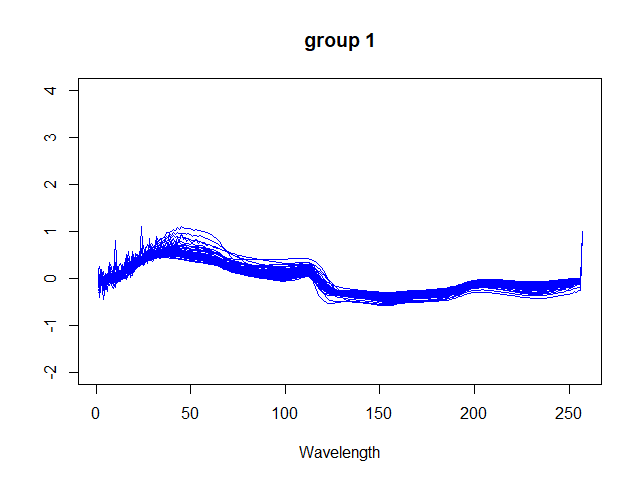
\includegraphics[width=\textwidth]{../images/project2/group1_wavelength.png}
   \caption{Spectral plot of group 1}\label{fig:group1_wavelength}
  \end{subfigure}%
  %
  \begin{subfigure}[b]{0.35\linewidth}
      \centering
   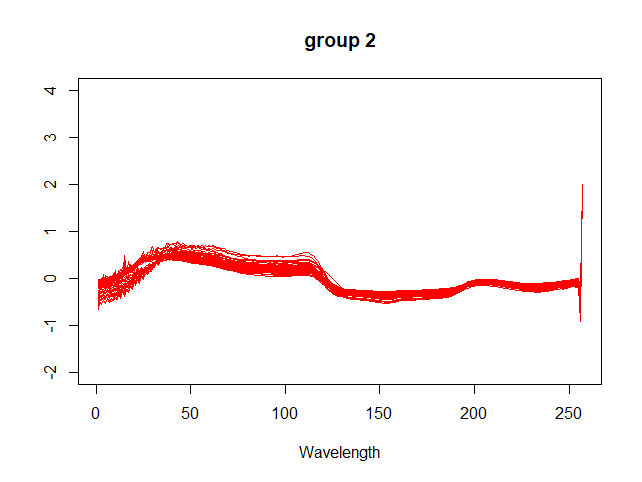
\includegraphics[width=\textwidth]{../images/project2/group2_wavelength.png}
   \caption{Spectral plot of group 2}\label{fig:group2_wavelength}
  \end{subfigure} \\%
  \begin{subfigure}[b]{0.35\linewidth}
    \centering
    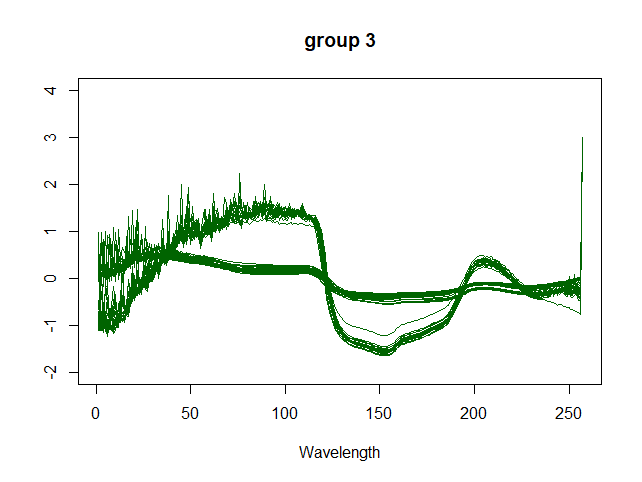
\includegraphics[width=\textwidth]{../images/project2/group3_wavelength.png}
 \caption{Spectral plot of group 3}\label{fig:group3_wavelength}
\end{subfigure}%
%
\begin{subfigure}[b]{0.35\linewidth}
    \centering
 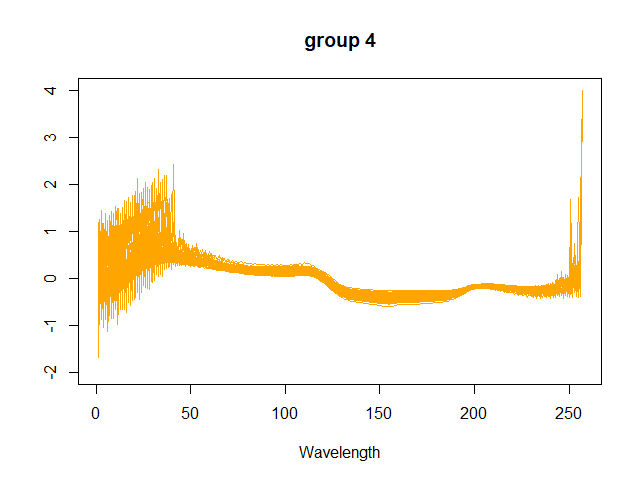
\includegraphics[width=\textwidth]{../images/project2/group4_wavelength.png}
 \caption{Spectral plot of group 4}\label{fig:group4_wavelength}
\end{subfigure}%
 \caption{Spectral plots by group}
 \label{spectralByGroup}
\end{figure}


\section{K-medoids clustering}

In the following sections we discuss results obtained by \textit{k-medoids} clustering method. We impose 2 up to 6 clusters to randomly drawn data.

\subsection{Evaluating cluster quality}
Without using the information we have on which group do individual observations belong to, we look into the quality of clusters obdatined. For this purpose we 
use \textit{silhouette values and plots}, that help us determine how similar are objects in a given cluster.

Starting off with two clusters already gives quite satisfying results. As seen in image \ref{fig:silhouette_pam2}, average silhouette width for the whole dataset is 0.76,
which indicates we have found strong structure in the data.
Some further analysis reveals that silhouette widths for each of the clusters are 0.76 and 0.79, respectively. We also see that the first cluster contains much more elements than
the second -- 182 compared to 18.

\begin{figure}[h]
  \begin{center}
    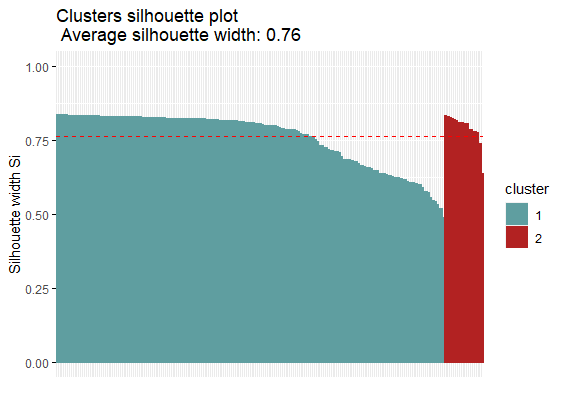
\includegraphics[width = 0.5\textwidth]{../images/project2/silhouette_pam2.png}
    \caption{Silhouette plot for two clusters}
    \label{fig:silhouette_pam2}
  \end{center}
\end{figure}

We continue with the clustering and quickly notice a negative trend, with silhouette values never reaching the heights from those obtained with two clusters.
Minimum is reached with four clusters, with the average silhouette width 0.29 and values for some individual observations falling below zero. More clusters also
result in one large main cluster and a few smaller ones.

These results can be summarised in figure \ref{fig:optNumber}, where we see a clear peak at $k=2.$
\begin{figure}
  \begin{center}
    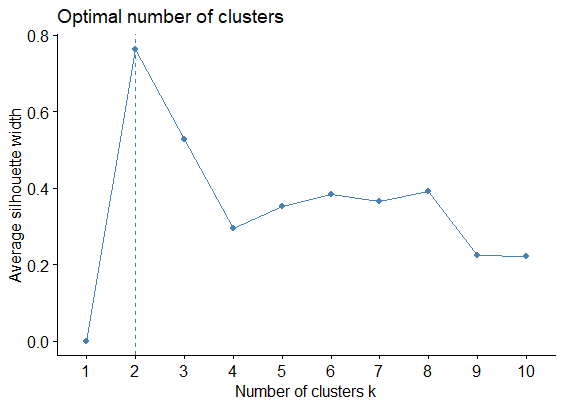
\includegraphics[width = 0.45\textwidth]{../images/project2/number_of_clusters.png}
    \caption{Average silhouette widths with different numbers of clusters}
    \label{fig:optNumber}
  \end{center}
\end{figure}

\subsection{Comparison of clustering with known groups}

Now we will also take into account the information we have on groups and investigate how they relate to our clustering methods. 

Confusion matrix for two clusters reveals, that the small second cluster completely consists of observations from group 3 (figure \ref{fig:confMat_2}) -- as predicted in the introduction. Additionally, making
more than 4 clusters results in observations from group 4 being spread out across more clusters and a part of groups 2 and 3 fall in clusters 2 and 3 respectively, as depicted in figures \ref{fig:confMat_4} and \ref{fig:confMat_6}.
We can already see the trend where clustering does not follow the underlying grouping.

\begin{figure}[h!]
  \begin{subfigure}[b]{0.33\linewidth}
      \centering
      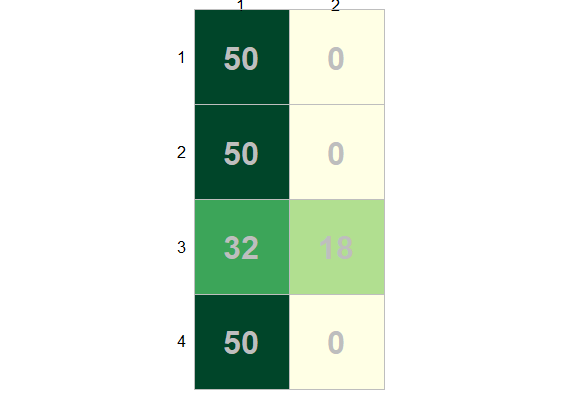
\includegraphics[width=\textwidth]{../images/project2/confMat_2.png}
   \caption{}\label{fig:confMat_2}
  \end{subfigure}%
  %
  \begin{subfigure}[b]{0.33\linewidth}
      \centering
   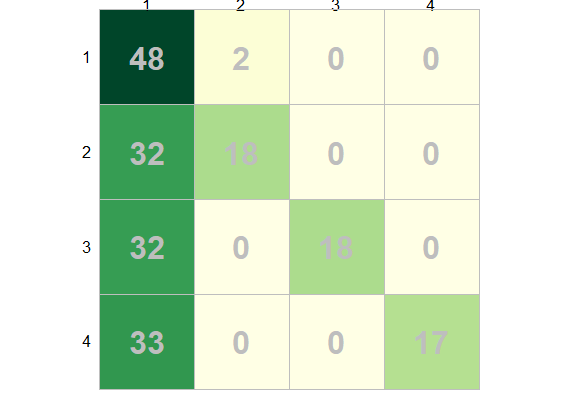
\includegraphics[width=\textwidth]{../images/project2/confMat_4.png}
   \caption{}\label{fig:confMat_4}
  \end{subfigure}%
  \begin{subfigure}[b]{0.33\linewidth}
    \centering
 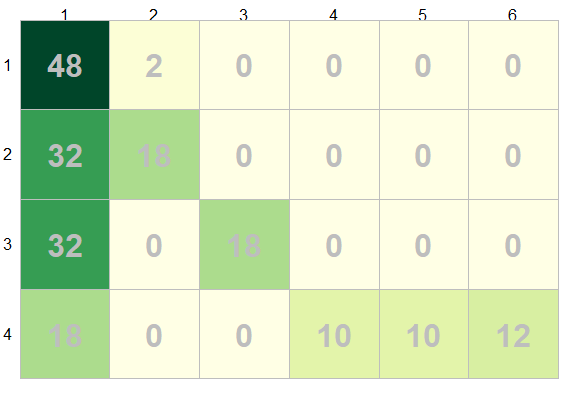
\includegraphics[width=\textwidth]{../images/project2/confMat_6.png}
 \caption{}\label{fig:confMat_6}
\end{subfigure}%
\caption{Confusion matrices for $k=2$, $k=4$ and $k=6$.}
\label{fig:confMat}
\end{figure}

Drawing cluster plots of PCA scores gives some additional insight into cluster structures. Plotting the results from two clusters in figure \ref{fig:clusPlot_pam2}
we see one larger group and one smaller, far away from the other. With more clusters generated, the large datacloud on the left gets divided further into smaller clusters, most of which are overlapping significantly, as seen in
\ref{fig:clusPlot_pam6}.

\begin{figure}[h]
  \begin{subfigure}[b]{0.5\linewidth}
      \centering
      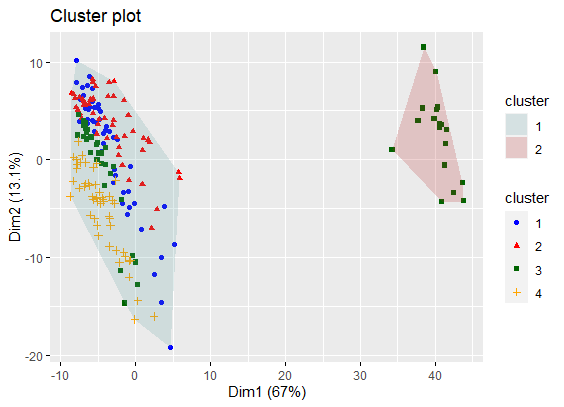
\includegraphics[width=\textwidth]{../images/project2/clusPlot_pam2.png}
   \caption{Cluster plot with $k=2$}\label{fig:clusPlot_pam2}
  \end{subfigure}%
  %
  \begin{subfigure}[b]{0.5\linewidth}
      \centering
   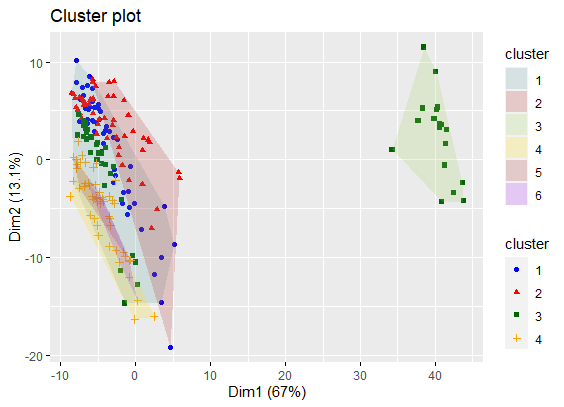
\includegraphics[width=\textwidth]{../images/project2/clusPlot_pam6.png}
   \caption{Cluster plot with $k=6$}\label{fig:clusPlot_pam6}
  \end{subfigure}%
 \caption{Cluster plots}
\end{figure}

Similar conclusion can be drawn by looking at spectral plots, coloured according to the clustering as seen in figure \ref{fig:spectraByClusters}. In figure \ref{fig:spectraByClusters_pam2}
clearly see that with $k=2$ we get separation between main group and the differently behaving one. Adding more groups divides the main group further, but there is no clear
structure.

\begin{figure}[h!]
  \begin{subfigure}[b]{0.33\linewidth}
      \centering
      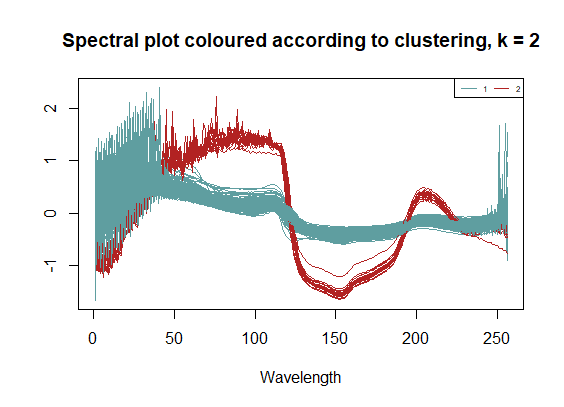
\includegraphics[width=\textwidth]{../images/project2/spectraByClusters_pam2.png}
   \caption{}\label{fig:spectraByClusters_pam2}
  \end{subfigure}%
  %
  \begin{subfigure}[b]{0.33\linewidth}
      \centering
   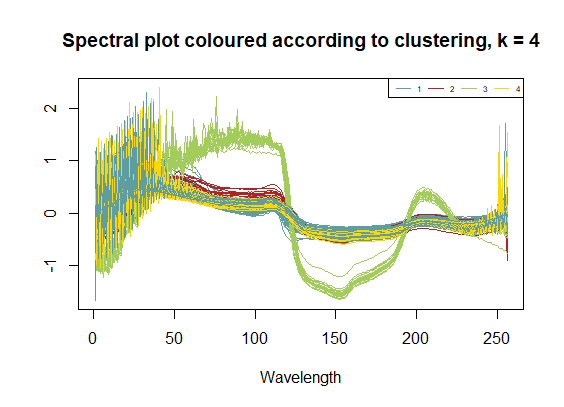
\includegraphics[width=\textwidth]{../images/project2/spectraByClusters_pam4.png}
   \caption{}\label{fig:spectraByClusters_pam4}
  \end{subfigure}%
  \begin{subfigure}[b]{0.33\linewidth}
    \centering
 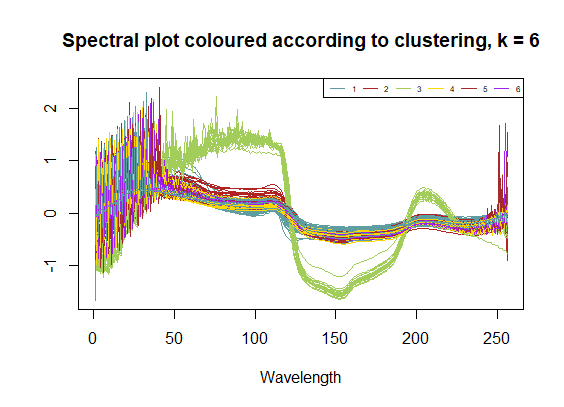
\includegraphics[width=\textwidth]{../images/project2/spectraByClusters_pam6.png}
 \caption{}\label{fig:spectraByClusters_pam6}
\end{subfigure}%
\caption{Spectral plots coloured according to clustering}
\label{fig:spectraByClusters}
\end{figure}

Other ways of analysing, such as heatmaps and mosaic plots do not reveal any new information on the clustering, so we do not include them in the report.
Based on all results above we conclude that the optimal number of clusters is $k_{opt} = 2$.

\section{Hierarchical clustering}

We continue our research by performing agglomerative hierarchical clustering with average and complete linkage. When considering hard clustering with $k_{opt}$ 
results are exactly equal to those obtained by k-medoids clustering -- Rand index of the clusterings is 1.
We can attribute this to the very clear structure in the data, with one group being rather far from another.

Looking at dendrograms of both clustering methods, we notice a very large jump in height when going from 3 to 2 clusters, and much smaller ones 
when the number of clusters is larger.

\begin{figure}[h]
  \begin{subfigure}[b]{0.5\linewidth}
      \centering
      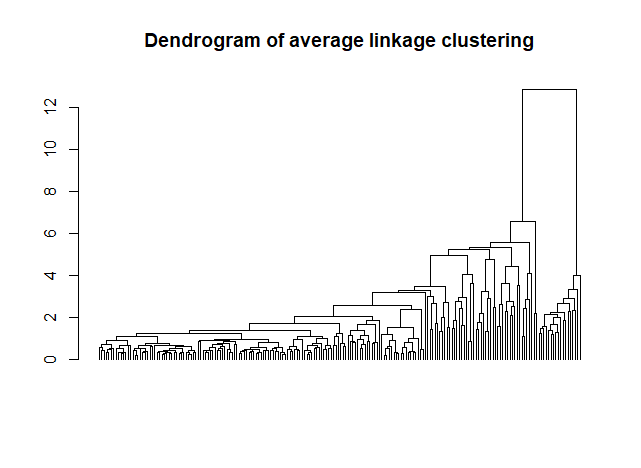
\includegraphics[width=\textwidth]{../images/project2/avgDend.png}
   \caption{Dendrogram of average linkage clustering}\label{fig:avgDend}
  \end{subfigure}%
  %
  \begin{subfigure}[b]{0.5\linewidth}
      \centering
   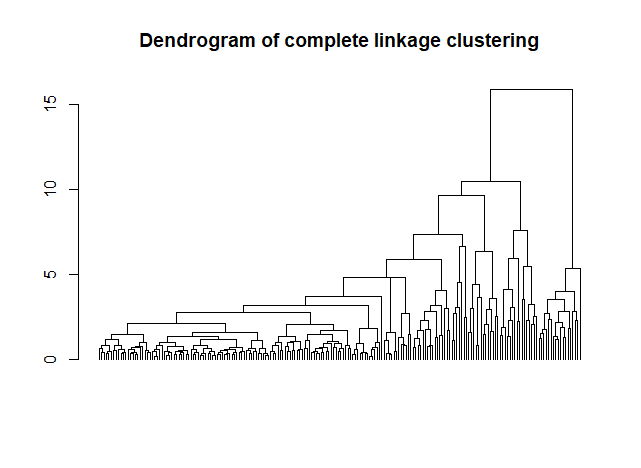
\includegraphics[width=\textwidth]{../images/project2/compDend.png}
   \caption{Dendrogram of complete linkage clustering}\label{fig:cmpDend}
  \end{subfigure}%
 \caption{Dendrograms of hierarchical clusterings}
\end{figure}

Further, taking complete linkage into account, we investigate a third group that seems to be appearing (visible on the right of dendrogram \ref{fig:cmpDend}). Hard clustering with
$k = 3$ results in a large drop of average silhouette value, which in this case equals 0.43. Plotting the cluster plot reveals that the new cluster contains
mostly data from the 4th group, however it almost completely overlaps with the second cluster. Calculating the contingency table for this clustering we find out
that the cluster plot decieves us a bit -- only 14 members of the 4th group are in a separate clusters while the others still remain in the large first cluster.
\begin{figure}[h]
  \begin{subfigure}[b]{0.5\linewidth}
      \centering
      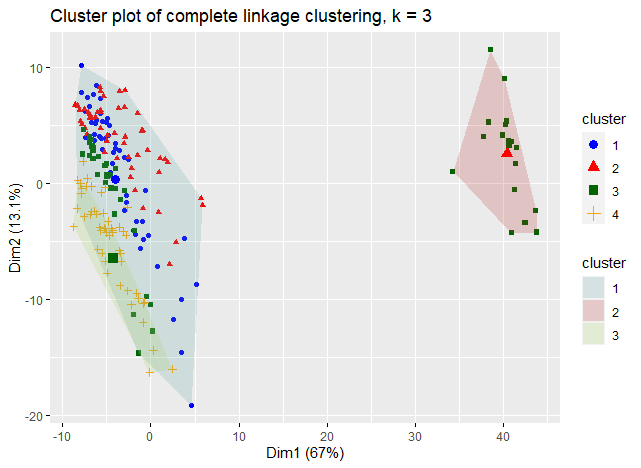
\includegraphics[width=\textwidth]{../images/project2/clusPlot_cmt3.png}
      \label{fig:clusPlot_cmt3}
      \caption{Cluster plot of hierarchical complete linkage clustering with 3 clusters}
  \end{subfigure}%
  %
  \begin{subfigure}[b]{0.5\linewidth}
      \centering
   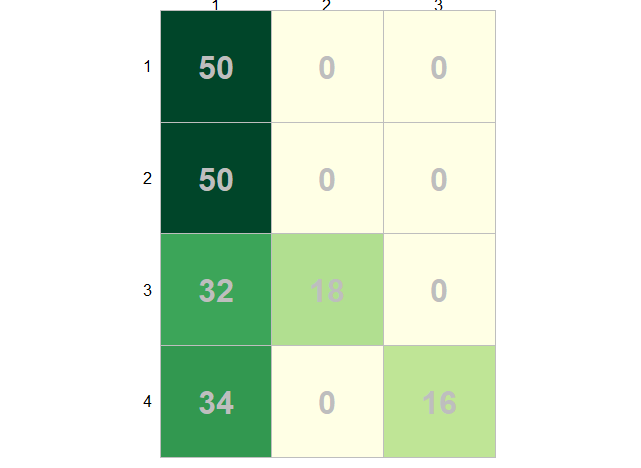
\includegraphics[width=\textwidth]{../images/project2/confMat_comp3.png}
   \caption{Confusion matrix of complete linkage clustering with $k=3$}\label{fig:confMat_comp3}
  \end{subfigure}%
 \caption{Analysis of complete linkage clustering with $k=3$}
\end{figure}

Finally, we compare k-medoids and hierarchical clusterings. In table \ref{tab:rand} we see that in most cases clusterings are quite similar, differing the most
when it comes to splitting the data into four clusters. In all cases except for 6 clusters, k-medoids is more similar
to complete linkage clustering than the two hierarchical methods.
%\begin{center}
  \begin{table}[h]
    \centering
  \begin{tabular}{ |c||c|c|c| } 
   \hline
   $k$ & complete, average  & k-med, average & k-med, complete \\
   \hline 
   2 & 1 & 1 & 1 \\ 
   3 & 0.881809 & 0.8741206 &0.9555276 \\ 
   4 & 0.7514573 &0.7020101 & 0.7801005 \\
   5 & 0.829598 &0.7288442 & 0.8322111 \\
   6 & 0.9221608 & 0.7720101& 0.8433166 \\
   \hline
  \end{tabular}
  \caption{Table of Rand indices}
  \label{tab:rand}
\end{table}
%\end{center}

\section{Conclusion}

We conclude that setting the number of clusters to two, both hierarchical and k-medoids clustering return same results, so either method is appropriate in this case.
This is true because of the data structure, which is clearly divisible in two groups. Splitting the clusters lowers the silhouette values in both cases, which 
are somewhat higher in hierarchical case as compared to k-medoids (they still fall well below 0.5 mark). Comparing all clustering methods also reveals that they do not
differ a lot, with pairwise Rand indices always staying above 0.7.

While clusters do not align perfectly with the groups from data, new clusters (when $k$ is less or equal than 4) consist of observations of separate groups -- but the majority of observations still remain in 
the first, largest cluster. Increasing the number of clusters to five or six results in splitting group 4 into smaller clusters, with other clusters remaining intact.

\end{document}